\chapter{Introdução}

Tendo em vista o desafio de prover Inclusão Digital, principalmente para
populações que não cresceram tendo acesso aos meios digitais, seja por falta de
recursos e oportunidade, seja por questões temporais, propomos o
desenvolvimento de uma plataforma educacional voltada para este público. A
ideia é prover cursos e guias de simples acesso para guiar o uso dos meios
digitais desde os primeiros fundamentos, promovendo instrução de uso,
conscientização e uma futura independência digital.

Sendo assim, tomamos como inspiração uma das maiores plataformas educacionais
de livre acesso hoje disponíveis, a \textit{Khan Academy}, porém mudando seu
propósito para além do mundo acadêmico e tentando enfatizar a acessibilidade
àqueles que não estão habituados aos meios digitais.

\chapter{Modelo Entidade-Relacionamento}

%%%%%%%%%%%%%%%%%%%%%%%%%%%%%%%%%%%%%%%%%%%%%%%%%%%%%%%%%%%%%%%%
% Requisitos

\section{Levantamento de Requisitos}

%%%%%%%%%%%%%%%%
% Autenticação %
%%%%%%%%%%%%%%%%

Um usuário do sistema poderá utilizar a plataforma de forma anônima (não
autenticada) ou de maneira identificável. Para que isso seja possível, um
usuário pode se cadastrar de maneira simples \textbf{\textit{(usuário
    autenticado)}}, inserindo apenas um \textbf{\underline{nome de usuário}} (3 a
16 caracteres), uma \textbf{senha} (que será armazenada como uma hash,
estimando 144 caracteres necessários para sua persistência) e, opcionalmente,
um \textbf{e-mail} (ocupando no máximo 254 caracteres). Além disso, para
moderar a plataforma e atualizá-la com mais conteúdos, teremos também
\textbf{\textit{usuários administrativos}}, esses são semelhante aos usuários
convencionais, sendo diferenciados por um booleano \textbf{admin}, além disso
todo administrador deve obrigatoriamente conter um e-mail cadastrado que será
utilizado para autenticação em dois fatores.

%%%%%%%%%%%%%%
% Banimentos %
%%%%%%%%%%%%%%

Um \textit{administrador} pode banir um usuário da plataforma, quando isso
ocorre temos a entidade de \textbf{\textit{banimento}}, nela são indicados: o
\textbf{\underline{responsável}} (referência ao administrador) responsável pelo
banimento, o \textbf{\underline{usuário banido}} (referência ao usuário
banido), o \textbf{\underline{horário}} (data e hora de criação), a
\textbf{validade} (data e hora em que o banimento expira) e, opcionalmente, a
\textbf{causa} (texto) do banimento. Administradores não podem ser banidos.

%%%%%%%%%%%%%
% Feedbacks %
%%%%%%%%%%%%%

A ideia é que esse seja um projeto dirigido e voltado para a comunidade, por
conta disso é bastante importante que usuários consigam prover
\textbf{\textit{feedbacks}}, sugerindo melhorias, apontando problemas
encontrados e solicitando novos tópicos. Esses feedbacks, então, terão uma
referência de qual é o \textbf{\underline{autor}} (referência ao usuário que
criou o feedback), o \textbf{\underline{horário}} (data e hora de criação do
feedback) a \textbf{mensagem} (texto de tamanho dinâmico, limitado
arbitrariamente à 4096 caracteres) e, opcionalmente, a \textbf{data de
  fechamento} (data e hora quando o feedback foi fechado). Além disso, a fim de
garantir a visualização dos feedbacks, temos uma entidade de
\textbf{\textit{visualização de feedback}}, ela associa um
\textbf{\underline{leitor}} (referência ao usuário administrador) e um
\textbf{\underline{feedback}} (referência ao feedback) junto à informação da
\textbf{\underline{data de visualização}} (data e hora quando a visualização
foi feita).

%%%%%%%%%%%%%%%
% Organização %
%%%%%%%%%%%%%%%

A fim de organizar o conteúdo, seguiremos uma divisão hierárquica bastante
comum, seguindo em: categorias, tópicos, unidades e conteúdos, do maior para o
menor, respectivamente. Primeiramente, teremos a \textbf{\textit{categoria}},
sendo o nível mais alto da hierarquia, ela é bastante simples, tendo apenas um
\textbf{\underline{nome}} (texto), uma \textbf{descrição} (texto) e um
\textbf{ícone} (url). Em sequência, temos os \textbf{\textit{cursos}}, que
contém um \textbf{\underline{nome}} (texto), uma \textbf{descrição} (texto) e a
\textbf{\underline{categoria}} (referência à categoria). Seguindo adiante,
teremos as \textbf{\textit{unidades}}, nosso próximo nível na hierarquia. As
unidades seguem uma estrutura similar, contendo um \textbf{\underline{nome}}
(texto), uma \textbf{descrição} (texto), sua \textbf{ordem} (inteiro), que é
usada para controlar a ordem em que as unidades são apresentadas, e o
\textbf{\underline{curso}} (referência à curso) a qual pertence. Por último
temos os \textbf{\textit{tópicos}}, eles são o nível mais baixo na hierarquia
organizacional, abrigando os conteúdos em si. Os tópicos seguem praticamente a
mesma estrutura das unidades, ou seja, possuem um \textbf{\underline{nome}}
(texto), uma \textbf{descrição} (texto), uma \textbf{ordem} (inteiro) e, por
fim, a \textbf{\underline{unidade}} (referência à unidade) a qual pertencem.

%%%%%%%%%%%%%
% Conteúdos %
%%%%%%%%%%%%%

Um dos principais elementos da plataforma, que seria a linha final desta
hierarquia, são os \textbf{\textit{conteúdos}}, todos os conteúdos terão alguns
campos em comum: um \textbf{\underline{título}} (texto), um \textbf{subtítulo}
(texto), uma \textbf{duração estimada} (inteiro indicando o número de minutos)
e o \textbf{\underline{tópico}} (referência ao tópico) a qual pertence. Além
disso, inicialmente, teremos três tipos de conteúdo: \textbf{\textit{artigos}},
que seriam conteúdos primariamente textuais, contendo, além dos comuns entre os
conteúdos, o \textbf{corpo} do artigo (que será um texto formatado em MD).
Teremos também, os \textbf{\textit{vídeos}}, que contém a \textbf{url} do vídeo
(texto) e uma \textbf{descrição} (texto) do vídeo. Por fim, teremos os
\textbf{\textit{exercícios}}, eles são compostos de um \textbf{enunciado
  (corpo)} (texto formato em MD) e o \textbf{limite de seleções de alternativas}
(inteiro indicando quantas alternativas um usuário pode selecionar). Além
disso, os \textit{exercícios} possuem um número variável de alternativas
associadas, cada \textbf{\textit{alternativa}} consiste de um
\textbf{\underline{corpo}} (texto formatado em MD), opcionalmente, uma
\textbf{explicação} (texto formatado em MD), se é uma alternativa
\textbf{correta} (booleano) e, por fim, o \textbf{\underline{exercício}}
(referência ao exercício) que faz parte.

%%%%%%%%%%%%%
% Histórico %
%%%%%%%%%%%%%

Para \textit{usuários autenticados}, será mantido um histórico do progresso
dele na plataforma, isto é: para cada \textit{conteúdo}, será registrado um
\textbf{\textit{evento de progresso}}, indicando o \textbf{\underline{horário}}
(data e hora) onde foi feito o progresso, qual o \textbf{\underline{conteúdo}}
(referência ao conteúdo) que foi visitado e, caso o conteúdo seja um
\textit{exercício}, as \textbf{alternativas selecionadas} (referências às
alternativas). Importante notar que as alternativas selecionadas precisam fazer
parte do conteúdo do tipo exercício referente ao evento. Os eventos de
progresso podem ser visualizados pelo usuário e podem existir mais de um evento
para o mesmo conteúdo. O usuário pode deletar eventos antigos a fim de
reiniciar o seu progresso de acordo com a granularidade desejada.

%%%%%%%%%%%%%%%
% Comentários %
%%%%%%%%%%%%%%%

Além disso, \textit{usuários autenticados}, podem deixar comentários em
conteúdos, cada \textbf{\textit{comentário}} é composto por um \textbf{corpo}
(texto em MD), o \textbf{\underline{autor}} (referência ao usuário que o
criou), o \textbf{\underline{conteúdo}} (referência ao conteúdo) em que o
comentário foi feito, o \textbf{\underline{horário}} (data e hora de criação)
em que o horário foi feito, se ele é \textbf{visível} (booleano indicando se
ele é exibido) para casos de deleção e, por fim, um comentário pode ser uma
resposta, nesses casos temos o campo de \textbf{comentário pai} (referência
opcional a um comentário) que indica qual comentário aquele responde. A
presença desse mecanismo de respostas cria uma restrição onde precisamos
garantir que, caso o comentário seja uma resposta, o conteúdo associado ao
comentário pai seja o mesmo que o conteúdo referenciado presente em si. Além
disso, a fim de evitar ciclos de relacionamento, precisamos garantir que, ao ir
seguindo a cadeia de comentários pai, não haja a existência de um ciclo no
momento da criação.

%%%%%%%%%%%
% Reports %
%%%%%%%%%%%

A fim de garantir a moderação da plataforma, \textit{usuários autenticados}
podem reportar comentários, para isso temos a entidade de
\textbf{\textit{report}}. Cada report consiste de um \textbf{\underline{autor}}
(referência ao usuário que fez o report), o \textbf{\underline{comentário
    reportado}} (referência ao comentário sendo reportado), o
\textbf{\underline{horário}} (data e hora de criação), o \textbf{motivo}
(texto) e, por fim, o indicador de \textbf{verificado} (booleano), que indica
que aquele report já foi avaliado por um administrador.

%%%%%%%%%%%%%%%%%%%%%%%%%%%%%%%%%%%%%%%%%%%%%%%%%%%%%%%%%%%%%%%%
% Funcionalidades

\section{Funcionalidades}

Analisando por cima dos atores do sistema, conseguimos sintetizar as
funcionalidades da plataforma da seguinte forma:

\begin{itemize}
  \item \textbf{Usuário Não Cadastrado}
        \begin{itemize}
          \item Cadastrar-se
          \item Navegar pelas categorias, cursos, tópicos, unidades e conteúdos
          \item Consumir os conteúdos
          \item Realizar exercícios
          \item Visualizar comentários de um conteúdo
        \end{itemize}
  \item \textbf{Usuário Cadastrado}
        \begin{itemize}
          \item \textit{(Todas de um Usuário Não Cadastrado)}
          \item Autenticar-se
          \item Alterar senha
          \item Atualizar e-mail
          \item Registrar (automaticamente) o progresso na plataforma
          \item Visualizar o progresso atual
          \item Reiniciar o progresso (de maneira granular)
          \item Criar comentários em um conteúdo (caso não esteja banido)
          \item Responder comentários existentes (caso não esteja banido)
          \item Reportar um comentário (caso não esteja banido)
          \item Deletar um próprio comentário
          \item Enviar feedbacks (caso não esteja banido)
        \end{itemize}
  \item \textbf{Usuário Administrador}
        \begin{itemize}
          \item \textit{(Todas de um Usuário Cadastrado)}
          \item Inserir, remover e atualizar: categorias, cursos, tópicos, unidades, artigos,
                aulas, exercícios e alternativas
          \item Deletar e atualizar comentários (de outros usuários)
          \item Banir e perdoar usuários cadastrados (que não sejam administradores)
          \item Visualizar os reports e comentários associados
          \item Marcar reports de um comentário como resolvido (todos até o momento atual)
          \item Visualizar feedbacks (histórico de visualização persistido)
          \item Marcar (ou desmarcar) feedback como resolvido (mantendo a data de resolução)
        \end{itemize}
\end{itemize}

%%%%%%%%%%%%%%%%%%%%%%%%%%%%%%%%%%%%%%%%%%%%%%%%%%%%%%%%%%%%%%%%
% Diagrama
\begin{landscape}
  \section{Diagrama do Modelo Entidade-Relacionamento}

  \begin{figure}[h]
    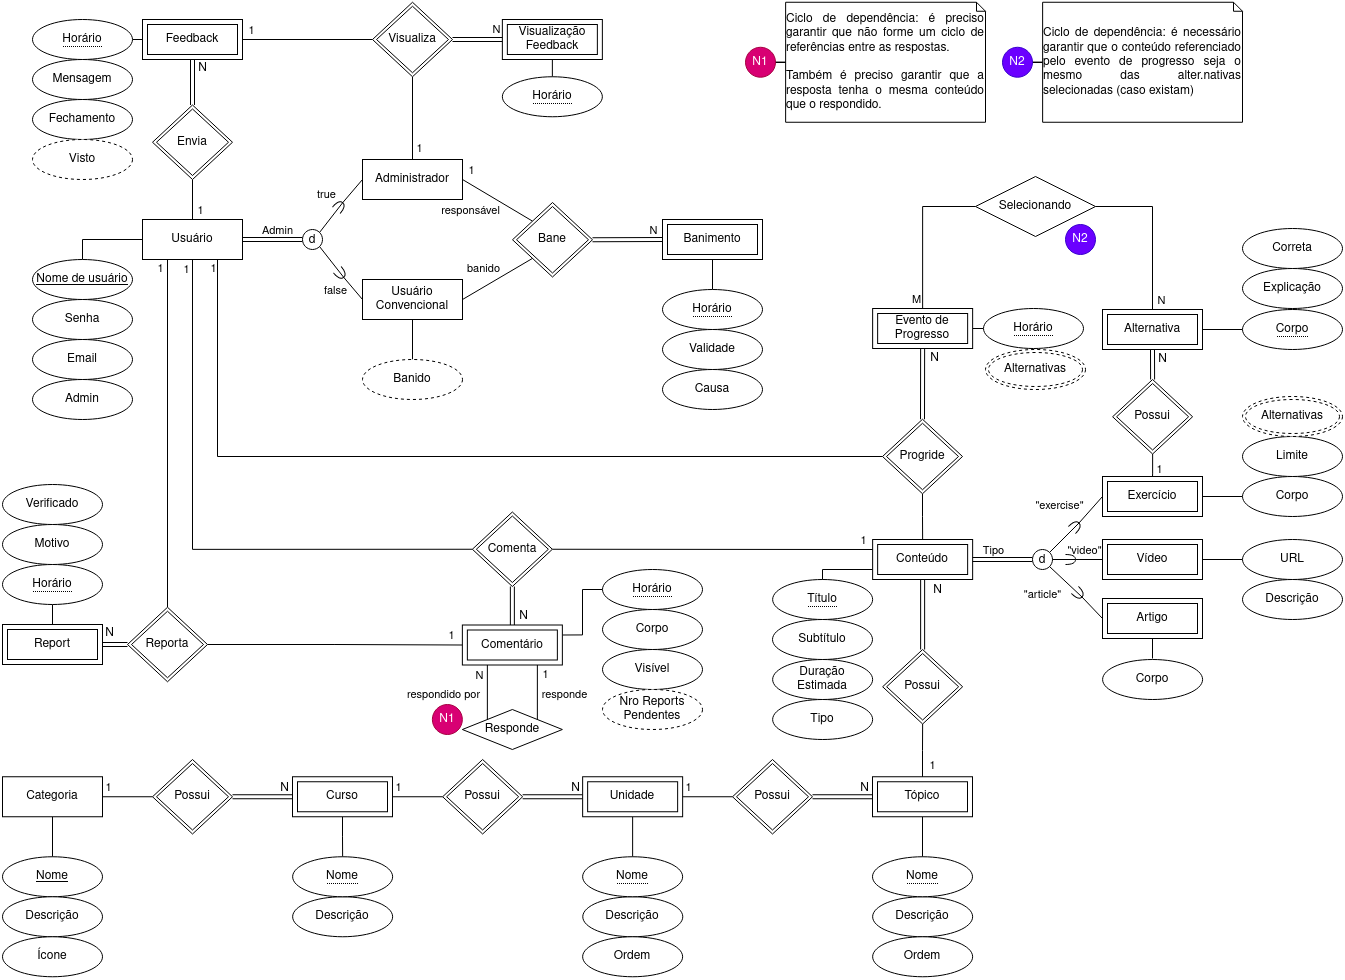
\includegraphics[height=0.76\textheight, center]{img/mer.png}
    \caption{Diagrama do Modelo Entidade-Relacionamento}
    \label{fig:mer}
  \end{figure}
\end{landscape}

%%%%%%%%%%%%%%%%%%%%%%%%%%%%%%%%%%%%%%%%%%%%%%%%%%%%%%%%%%%%%%%%
% Ciclos e restrições de integridade

\section{Ciclos e Restrições de Integridade}

A modelo proposto apresenta alguns ciclos naturais da solução e restrições de
integridade necessárias, trataremos-as individualmente a seguir:

\subsection{Ciclo: Comentário (Resposta) $\rightarrow$ Comentário (Respondido)}

Este é um dos ciclos mais complicados do diagrama, ele se trata de um ciclo de
dependência natural da modelagem, para solucioná-lo precisaremos garantir que
duas restrições sejam satisfeitas:

\begin{enumerate}
  \item Ao criar uma resposta, precisamos garantir que a referência de conteúdo do
        comentário respondido seja a mesma da resposta sendo criada.
  \item Ao criar uma resposta, precisamos garantir que, ao seguir a cadeia de
        comentários pais, não haja repetição de comentários (evitar ciclos, ex: $C_1
          \rightarrow \rightarrow C_2 \rightarrow C_3 \rightarrow C1$). É possível
        garantir isso ao impedir que o campo de comentário respondido seja editável.
\end{enumerate}

\subsection{Ciclo: Usuário $\rightarrow$ Comentário $\rightarrow$ Report}

Este é um ciclo natural da modelagem, não é necessário nenhum tratamento
especial, já que apenas indica a possibilidade (irônica) de um usuário reportar
o próprio comentário.

\subsection{Ciclo: Administrador $\rightarrow$ Feedback $\rightarrow$ Visualização Feedback}

Mais um ciclo natural do diagrama, no sistema optamos por não restringir o
administrador de fazer a maior parte das interações que um usuário convencional
faria, sendo assim, caso um administrador crie um feedback, existe a
possibilidade de que ele visualize o próprio feedback. Não é necessário nenhum
tratamento adicional neste caso.

\subsection{Ciclo: Conteúdo $\rightarrow$ Evento de Progresso $\rightarrow$ Alternativa}

Este é um ciclo natural do diagrama, ele até poderia ser evitado por meio de
uma especialização do Evento de Progresso, mas acreditamos que isso criaria uma
complexidade desnecessária na modelagem sem benefícios práticos. Consistindo de
um ciclo de dependência onde um Evento de Progresso, pode, opcionalmente, ter
referências a alternativas selecionadas. Quando isso acontece, é necessário
garantir que o conteúdo que a alternativa referencia (do tipo Exercício) seja o
mesmo que é referenciado pelo Evento de Progresso, originando, então, uma
restrição de integridade para que no momento de cadastro das alternativas
associadas ao evento de progresso, seja verificada essa igualdade dos conteúdos
referenciados.

\subsection{Restrição adicional: Administradores precisam de um E-mail cadastrado}

Para que um usuário se torne um administrador (campo admin igual a true), é
necessário que seu campo de email não seja nulo, criando assim a necessidade de
uma restrição de integridade adicional.

\subsection{Restrição adicional: Administradores não podem ser banidos}

Usuários administradores não podem ser banidos, por conta disso é necessário
uma restrição de integridade que garanta que usuários banidos não se tornem
administradores e que banimentos não sejam criados para administradores. É
possível evitar isso também ao impedir que usuários existentes não se tornem
administradores e nem administradores tornem-se usuários convencionais, mas não
pretendemos seguir por este caminho.
